Come detto nella sezione precedente, CUTE individua itemset chiusi, SPARE massimali.
Per quanto molti passi nei due approcci divergano, è possibile in determinate condizioni ottenere gli stessi risultati tra i due algoritmi.
Ciò però avviene solo in casistiche particolari, nella maggior parte delle situazioni succede che i risultai divergano per alcune caratteristiche intrinseche dei due algoritmi:

\begin{itemize}
    \item \textit{Itemset chiusi \(\supseteq\) Itemset massimali}. È fisiologico, salvo rare eccezioni, che il numero di itemset chiusi in un dataset sia anche di ordini di grandezza più grande di quello dei massimali.
    \item \textit{Le metriche spaziali divergono}.
   L'impiego di due metriche spaziali differenti porta a risultati che in assoluto possono divergere per alcune tuple.
\end{itemize}

Per quanto i due algoritmi possano avere elementi in comune, queste particolarità devono essere tenute in conto durante il confronto dei risultati.
Confrontare il numero di itemset identici produrrebbe quindi scarsi risultati.
Serve perciò definire una metrica di confronto che tenga conto di queste due caratteristiche: non deve penalizzare eccessivamente la differenza nel numero dei risultati e deve misurare la similarità tra gli itemset tenendo conto che questi possono divergere per l'assenza o presenza di qualche elemento.

Alla luce di questo, è stata formulata la seguente misura di similarità \(S\).
Per confrontare i due insiemi di itemset si utilizza una variazione dello Stable Marriage Problem~\cite{mcvitie1971stable}.
Dati due set di stesse dimensioni, questa tecnica permette di assegnare ogni elemento di un set a uno dell'altro sulla base di un criterio di similarità custom.
Questo permette di ottenere una soluzione sub-ottima al problema dell'assegnamento, assicurandosi che non esistano due elementi appartenenti a insiemi diversi che abbiano una similarità maggiore tra di loro rispetto che coi rispettivi partner (\cref{definition:stable-marriage-problem}).

\begin{definition}[Stable Marriage Problem]\label{definition:stable-marriage-problem}

 Dati due insiemi di oggetti \(N\) e \(M\), si definisce problema del matrimonio stabile il problema che ricerca l'insieme delle coppie \((n_i \in N, m_j \in M)\) tali che definita una metrica di similarità \(s\) non esistano in contemporanea due coppie \((n_p, m_p),(n_q,m_q)\) tali che  \(n_p,n_q \in N,m_p,m_q \in M\) per cui vale che: 
  \begin{center}
  \(
    \begin{cases}
     s(n_p,m_j) > s(n_i, m_j) \land s(n_p,m_j) > s(n_p,m_p) \\
     s(n_i, m_q) > s(n_i, m_j) \land s(n_i, m_q) > s(n_q, m_q)
    \end{cases}
    \)
  \end{center}
\end{definition}

Definita la modalità di assegnamento, si rende necessario individuare una metrica di confronto tra i singoli itemset.
Questa è definita via coefficiente di Jaccard.
Questo calcola la similarità tra due set come il numero di elementi condivisi tra i due diviso l'unione di tutti gli elementi presenti in entrambi (\cref{definition:jaccard}).

\begin{definition}[Coefficiente di Jaccard]\label{definition:jaccard}

 Dati due set di item \(N\) e \(M\), si definisce il coefficiente di Jaccard tra i due insiemi come: 
    \begin{center}
        \(Jaccard(N,M) = \frac{|N \cap M|}{|N \cup M|}\) 
    \end{center}
\end{definition}

Una volta definita questa metrica, la similarità totale \(S\) tra i risultati di CUTE e SPARE viene calcolata nel seguente modo:
in primo luogo viene eseguito l'assegnamento di ogni cluster individuato su un algoritmo a quello di un altro sulla base del valore di Jaccard tra i due.
Questa operazione segue le regole del problema del matrimonio stabile, di conseguenza produce una soluzione sub-ottima.
A questo punto viene calcolata la somma totale dei valori di similarità tra ogni coppia e questo risultato viene poi diviso per il numero delle coppie totali.
Il risultato di questa operazione determina la similarità tra due insiemi.

\begin{definition}[Similarità tra due set di cluster]\label{definition:cluster-similarity}

Dato un set di cluster di CUTE \(C\), uno di SPARE \(M\) e insieme di coppie \(CM = \{(c_1, m_1), \ldots, (c_n, m_n)\}\), generato mediante risoluzione del problema del matrimonio stabile utilizzando \(Jaccard\) come metrica di similarità, tali che \( c_ i \in C \land m_i \in M\) si definisce la similarità \(S\) con la seguente formula:

  \begin{equation}
     S(C, M) = \frac{\sum_{k=1}^{n}{Jaccard(c_k, m_k)}}{n} 
    \end{equation}

\end{definition}

Occorre però un'ulteriore precisazione.
Come detto sopra il problema del matrimonio stabile funziona solo se entrambi gli insiemi hanno lo stesso numero di elementi.
CUTE e SPARE invece divergono per numero di itemset: in particolare CUTE individuerà in media molti più risultati di SPARE.
Per risolvere questo problema, sono state definite due variazioni della metrica: in una gli elementi in più sono scartati \((S_{minus})\) mentre nell'altra \((S_{plus})\) contribuiscono alla misura con un valore di similarità pari a \(0\).
Tra queste due metriche ci è sembrato più rilevante cercare di massimizzare \((S_{minus})\), in quanto misura che penalizza in maniera minore la differenza di cardinalità tra massimali e chiusi.

Definita la procedura di confronto, è stato scelto come dataset utilizzato Oldenburg, campionato ogni \(5\) istanti temporali.
Questa configurazione garantisce che il numero di celle create da CUTE aumenta in maniera controllata, allo stesso tempo il dataset rimane abbastanza compatto per ottenere risultati significativi rispetto a SPARE.

I primi test sono stati condotti sul dataset nella sua interezza, a parità di risorse fornite.
CUTE sin da subito è stato in grado di gestire la complessità del problema nel suo insieme, mentre SPARE no.
In numerose occasioni, le risorse fornite all'applicazione non sono state sufficienti per permettere all'algoritmo di terminare con successo.

Alla luce di questi fallimenti, è stato ridotto il numero di traiettorie impiegate.
Sono stati così condotti esperimenti su \(1000, 2000\) e infine \(3000\) traiettorie.
Anche in queste condizioni, SPARE ha avuto difficoltà nell'eseguire la ricerca con determinate configurazioni.
Inoltre la differenza tra i risultati dei due algoritmi risultava decisamente grande: in alcune situazioni SPARE individuava \(1\text{-}2\) elementi, mentre CUTE sui \(1000\text{-}2000\).

Sono state impiegate allora tecniche e accorgimenti per riuscire a ottenere risultati significativi.
Il primo passo è stato individuare una configurazione di \(\epsilon, minPts\) che permettesse a SPARE di individuare un numero consistente di itemset (\(> 50\)) su più configurazioni.
Successivamente è stato lanciato diverse volte CUTE, variando il lato spaziale delle celle su valori ragionevoli e direttamente collegati a \(\epsilon\).
Di seguito (\cref{fig:chap-4:CompM,fig:chap-4:CompK,fig:chap-4:CompG,fig:chap-4:CompS}) è illustrato il confronto tra SPARE e CUTE.
La \cref{tab:comparison-variation} riassume le configurazioni di parametri in gioco.

\begin{table}[H]
    \centering
   \begin{tabular}{||c c c||}
 \hline
     Parametro & Algoritmo & Valori \\ [0.4ex] 
 \hline\hline
   \(s\) & CUTE & \(1.5,\textbf{1.75},2\) KM \\
 \hline
  \(\epsilon\) & SPARE & \(\textbf{2}\) KM \\
 \hline
 \(minPoints\) & SPARE & \(\textbf{5}\) \\
 \hline
 \(m\) & SPARE e CUTE & \(3,\textbf{4},5\) \\
 \hline
 \(k\) & SPARE e CUTE & \(4,\textbf{5},10\) \\
 \hline
 \(g\) & SPARE e CUTE & \(2,\textbf{5},1000\) \\
 \hline
\end{tabular}
    \caption{Valori dei parametri in gioco durante il confronto (default in grassetto)}
    \label{tab:comparison-variation}
\end{table}

\begin{figure}
  \centering
   \begin{subfigure}{.5\textwidth}
  \centering
      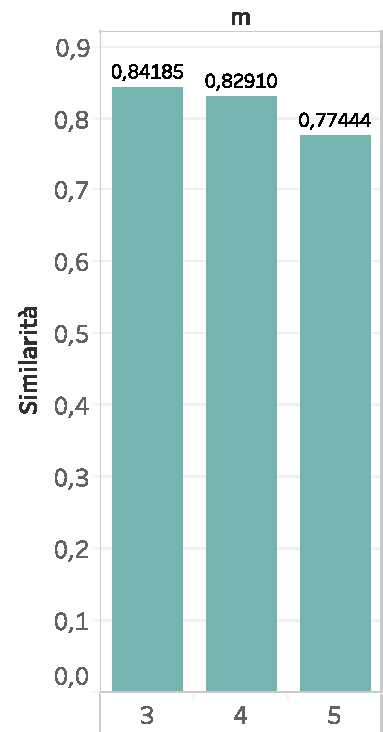
\includegraphics[scale=0.6]{res/fig/sec-4/scalability/ComparisonMSimilarity.pdf}
  \caption{Similarità \(S_{minus}\)}%
\end{subfigure}%
\begin{subfigure}{.5\textwidth}
  \centering
   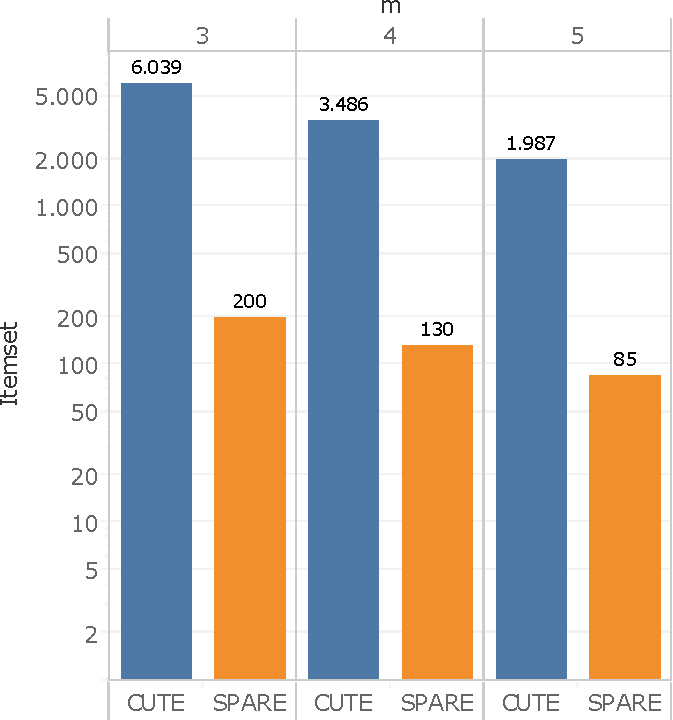
\includegraphics[scale=0.6]{res/fig/sec-4/scalability/ComparisonMCUTESPARE.pdf}
  \caption{Itemset individuati su CUTE e SPARE}%
  \end{subfigure}%
  \caption{Similarità a sinistra, itemset a destra al variare della dimensione minima dei gruppi \(m\)}%
  \label{fig:chap-4:CompM}
\end{figure}

\begin{figure}
  \centering
   \begin{subfigure}{.5\textwidth}
  \centering
      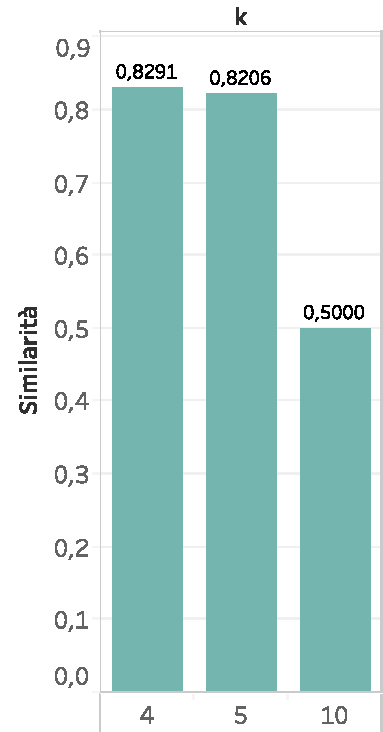
\includegraphics[scale=0.6]{res/fig/sec-4/scalability/ComparisonKSimilarity.pdf}
  \caption{Similarità \(S_{minus}\)}%
\end{subfigure}%
\begin{subfigure}{.5\textwidth}
  \centering
   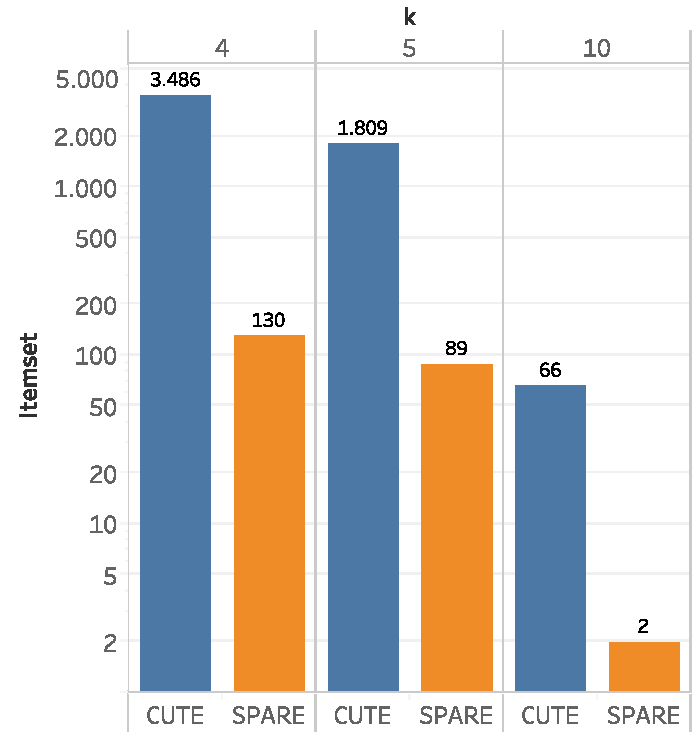
\includegraphics[scale=0.6]{res/fig/sec-4/scalability/ComparisonKCUTESPARE.pdf}
  \caption{Itemset individuati su CUTE e SPARE}%
  \end{subfigure}%
  \caption{Similarità a sinistra, itemset a destra al variare del supporto minimo \(k\)}%
  \label{fig:chap-4:CompK}
\end{figure}


Al variare di \(m\) (\cref{fig:chap-4:CompM}), è possibile vedere come all'aumentare delle dimensioni dei gruppi, la similarità totale tenda a calare.
Discorso analogo vale per \(k\): al suo aumentare la similarità totale cala.
Questo può essere giustificato sulla base delle divergenze nel determinare la vicinanza spaziale tra i due algoritmi.
Impostando infatti vincoli più rigidi, verranno riconosciuti itemset con maggiori dimensioni e supporto.
All'aumento di queste due misure corrisponde un incremento della possibilità che la composizione dei gruppi individuati tra i due algoritmi cambi.

Trattando invece di \(g\) \cref{fig:chap-4:CompG}, al rilassamento della continuità aumenta la similarità.
Anche questo è collegato con quanto detto sopra: pattern swarm contenenti gli stessi oggetti possono essere individuati in situazioni differenti.
È più raro che ciò possa accadere invece con pattern continui nel tempo, come ad esempio flock.

\begin{figure}
  \centering
   \begin{subfigure}{.5\textwidth}
  \centering
      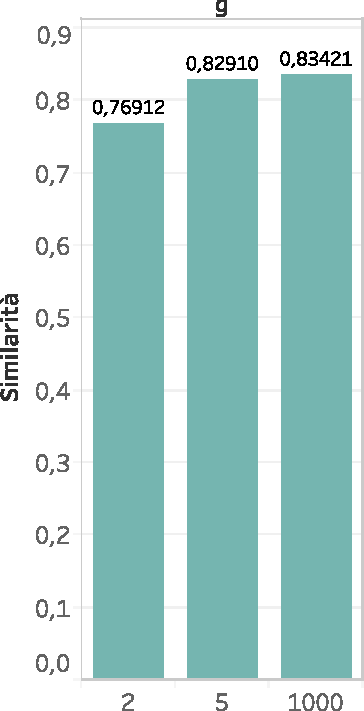
\includegraphics[scale=0.6]{res/fig/sec-4/scalability/ComparisonGSimilarity.pdf}
  \caption{Similarità \(S_{minus}\)}%
\end{subfigure}%
\begin{subfigure}{.5\textwidth}
  \centering
   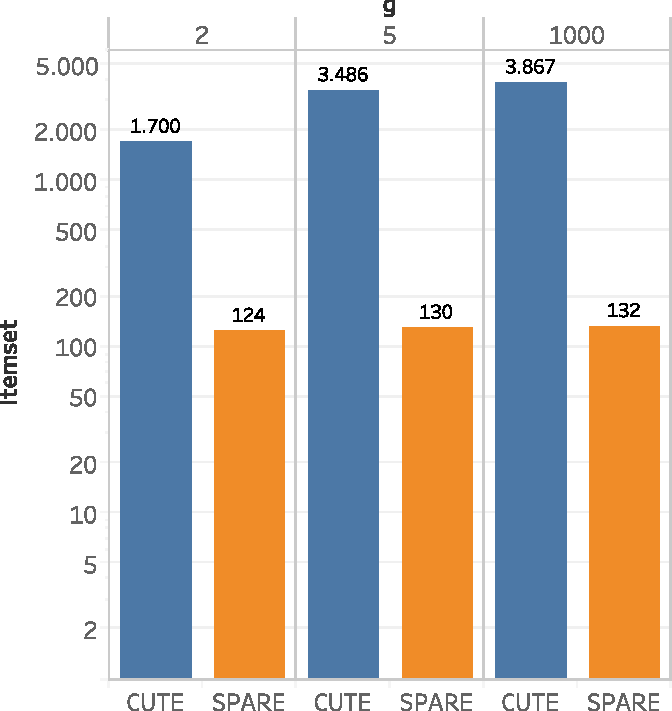
\includegraphics[scale=0.6]{res/fig/sec-4/scalability/ComparisonGCUTESPARE.pdf}
  \caption{Itemset individuati su CUTE e SPARE}%
  \end{subfigure}%
  \caption{Similarità a sinistra, itemset a destra al variare della continuità sul tempo \(g\)}%
  \label{fig:chap-4:CompG}
\end{figure}

Infine al variare di \(s\) si può vedere come il valore di similarità migliore si ottenga con il valore medio di \(s\).
La spiegazione di ciò può essere ricondotta alla distribuzione dei dati nello spazio.
Purtroppo è difficile determinare con precisione il valore ottimale di \(s\), se non determinandolo sperimentalmente.
Nonostante questo, \(1.75\) risulta un buon valore: quasi il \(50\%\) degli itemset di SPARE sono coperti da CUTE e la similarità complessiva è dell'\(80\%\). 

\begin{figure}
  \centering
   \begin{subfigure}{.5\textwidth}
  \centering
      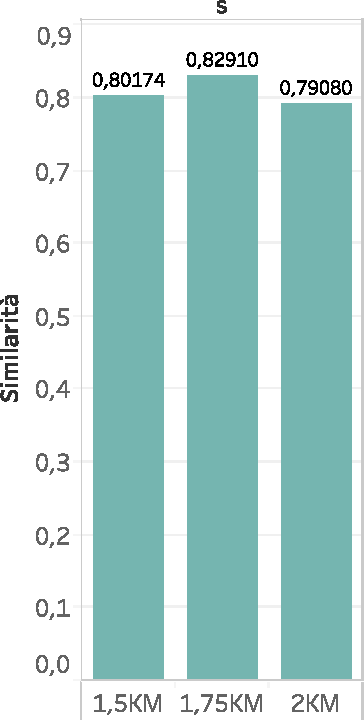
\includegraphics[scale=0.6]{res/fig/sec-4/scalability/ComparisonSSimilarity.pdf}
  \caption{Similarità \(S_{minus}\)}%
\end{subfigure}%
\begin{subfigure}{.5\textwidth}
  \centering
   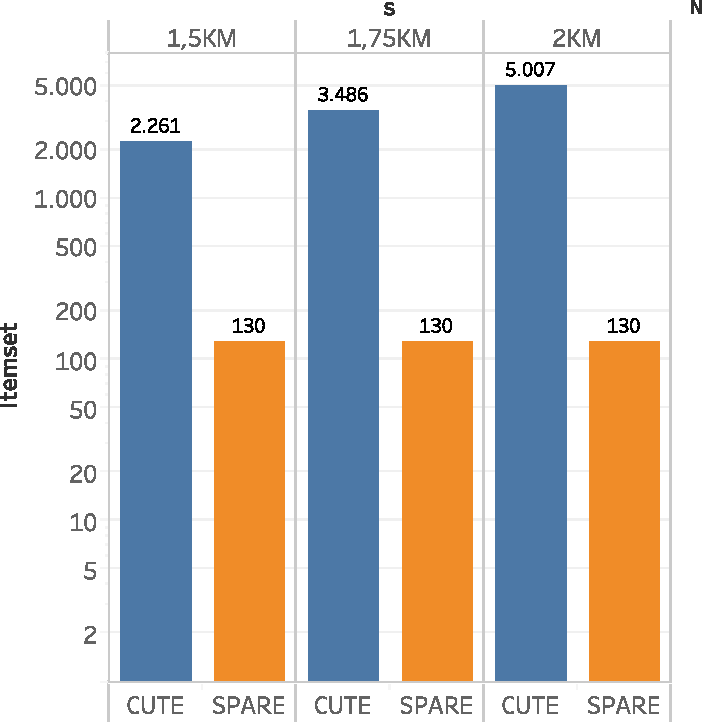
\includegraphics[scale=0.6]{res/fig/sec-4/scalability/ComparisonSCUTESPARE.pdf}
  \caption{Itemset individuati su CUTE e SPARE}%
  \end{subfigure}%
  \caption{Similarità a sinistra, itemset a destra al variare dell'area spaziale coperta dalle celle \(s\)}%
  \label{fig:chap-4:CompS}
\end{figure}
